\begin{example}~
\label{ex:single_noisy}
 	Consider a case where the set of confidential information is represented as $P = \set{(1,3),(2,1),(3,4),(4,1),(5,5),(6,9)}$. Suppose that \AgentOne sends this information on a single communication channel encrypted as $Q = \set{(1,12),(2,1),\\(3,16),(4,1),(5,17),(6,18)}$. In order to mask the transmitted information, \AgentOne sends adds noise to the communication channel by some noise relation represented by~$S$. \newline 

	We define the relations $P$ and $Q$ in \relview\ as follows: \newline

	\begin{figure}[ht]
		\centering
		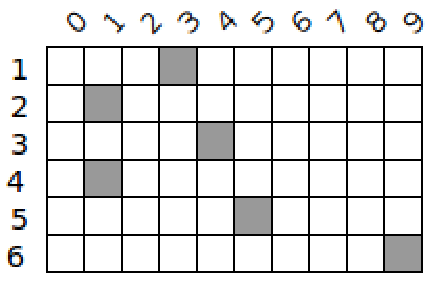
\includegraphics[scale=0.65]{Figures/PDF/Relview/P.pdf}
		\caption{Relation $P$ for Example~\ref{ex:single_noisy}.}
		\label{fig:single_noisy_p}
	\end{figure}
	\begin{figure}[ht]
		\centering
		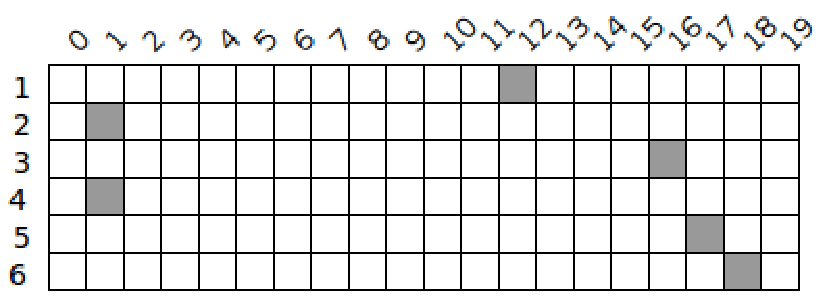
\includegraphics[scale=0.65]{Figures/PDF/Relview/Q.pdf}
		\caption{Relation $Q$ for Example~\ref{ex:single_noisy}.}
		\label{fig:single_noisy_q}
	\end{figure}

	Let the noise relation represented by $S$ be as follows: \newline

	\begin{figure}[ht]
		\centering
		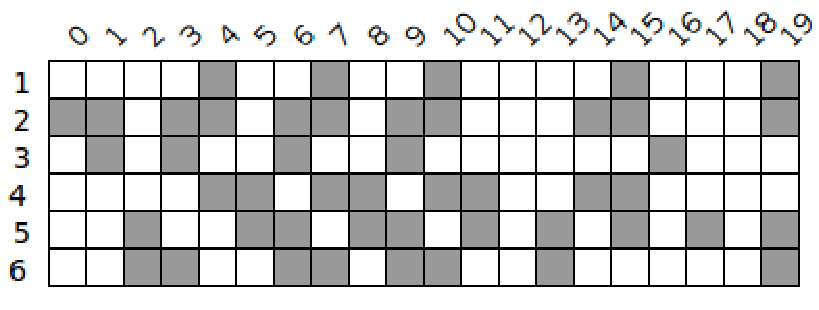
\includegraphics[scale=0.65]{Figures/PDF/Relview/NoiseQ.pdf}
		\caption{Noise relation $S$ for Example~\ref{ex:single_noisy}.}
		\label{fig:single_noisy_s}
		\end{figure}	
		
	\newpage
	We assume that the noise is added to the communication channel by the union operation ( $\!\!\!\STjoin\!\!\!$ ). The relation representing the noisy channel is then as follows:
	
	\begin{figure}[ht]
		\centering
		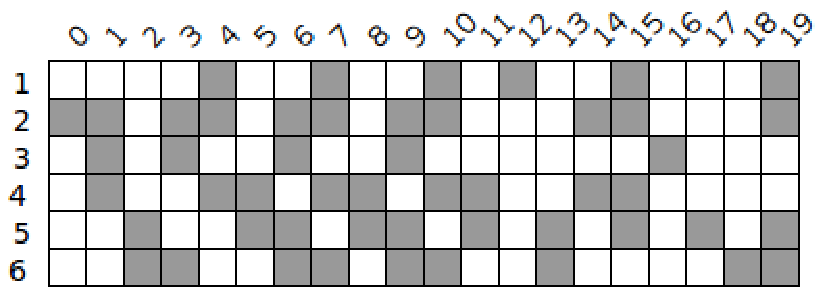
\includegraphics[scale=0.65]{Figures/PDF/Relview/QNoiseQ.pdf}
		\caption{Relation $Q \STjoin S$ for Example~\ref{ex:single_noisy}.}
		\label{fig:single_noisy_qs}
	\end{figure}

	We verify the existence of an abstraction relation by executing Program~\ref{prog:test} ($Result = Test(P, (Q \STjoin S))$). \newline

	\begin{figure}[ht]
		\centering
		
\includegraphics[scale=0.65]{Figures/PDF/Relview/True.pdf}
		\caption{Relation $Result$ for Example~\ref{ex:single_noisy}.}
		\label{fig:single_noisy_result}
	\end{figure}

	Therefore, the test has passed so we can compute the abstraction relation by executing Program~\ref{prog:compute} ($X = Compute(P,(Q \STjoin S),R)$) where $R$ is the filtering relation. \newline

	\begin{figure}[ht]
		\centering
		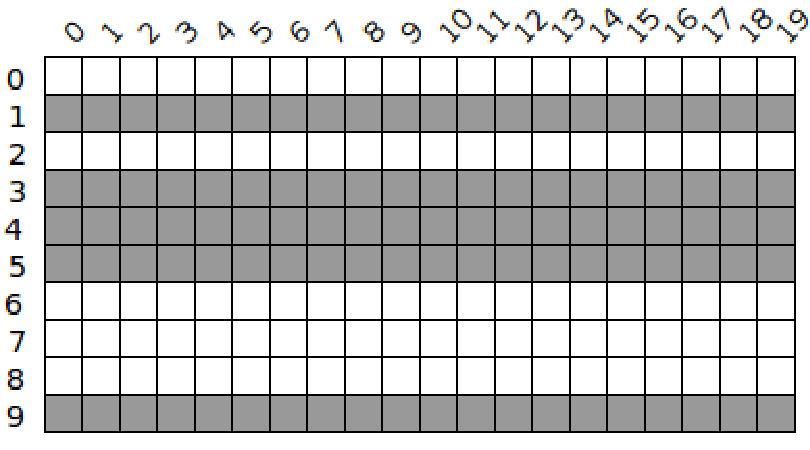
\includegraphics[scale=0.65]{Figures/PDF/Relview/R.pdf}
		\caption{Filtering relation $R$ for Example~\ref{ex:single_noisy}.}
		\label{fig:single_noisy_r}
	\end{figure}

	\begin{figure}[ht]
		\centering
		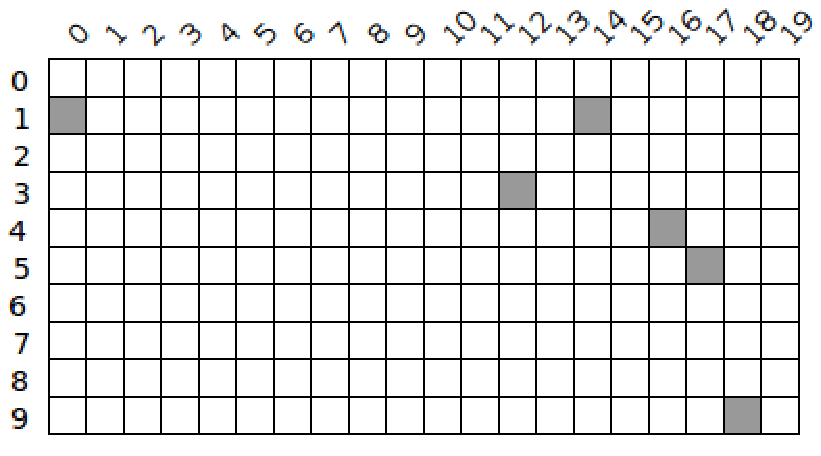
\includegraphics[scale=0.65]{Figures/PDF/Relview/XNQ.pdf}
		\caption{Abstraction relation $X$ for Example~\ref{ex:single_noisy}.}
		\label{fig:single_noisy_x}
	\end{figure}

	\newpage
\end{example}